\documentclass[a4paper,12pt]{article}

%Мои доработки
\usepackage[margin=10pt,font=small,labelfont=bf,
labelsep=period]{caption} % позволяет центровать подписи и издеваться над caption
%\usepackage{float} %здесь здесь, только здесь
\usepackage{floatrow} %нельзя одновременно включать floatrow и float
\usepackage{graphicx} %два пакета для размещения картинки и таблицы в ряд
%%% Работа с русским языком
\usepackage{enumitem} % развлекаться со списками
% объявляем новую команду для переноса строки внутри ячейки таблицы
\newcommand{\specialcell}[2][c]{%
	\begin{tabular}[#1]{@{}c@{}}#2\end{tabular}}
%	\renewcommand{\arraystretch}{1.8} %% increase table row spacing
%	\renewcommand{\tabcolsep}{1cm}   %% increase table column spacing


\usepackage{cmap}					% поиск в PDF
\usepackage{mathtext} 				% русские буквы в формулах
\usepackage[T2A]{fontenc}			% кодировка
\usepackage[utf8]{inputenc}			% кодировка исходного текста
\usepackage[english,russian]{babel}	% локализация и переносы

%%% Дополнительная работа с математикой
\usepackage{amsmath,amsfonts,amssymb,amsthm,mathtools} % AMS
\usepackage{icomma} % "Умная" запятая: $0,2$ --- число, $0, 2$ --- перечисление

%% Номера формул
%\mathtoolsset{showonlyrefs=true} % Показывать номера только у тех формул, на которые есть \eqref{} в тексте.
%\usepackage{leqno} % Нумерация формул слева

%% Свои команды
\DeclareMathOperator{\sgn}{\mathop{sgn}}

%% Перенос знаков в формулах (по Львовскому)
\newcommand*{\hm}[1]{#1\nobreak\discretionary{}
	{\hbox{$\mathsurround=0pt #1$}}{}}

%%% Работа с картинками
\usepackage{graphicx}  % Для вставки рисунков
\graphicspath{{images/}{images2/}}  % папки с картинками
\setlength\fboxsep{3pt} % Отступ рамки \fbox{} от рисунка
\setlength\fboxrule{1pt} % Толщина линий рамки \fbox{}
\usepackage{wrapfig} % Обтекание рисунков текстом

%%% Работа с таблицами
\usepackage{array,tabularx,tabulary,booktabs} % Дополнительная работа с таблицами
\usepackage{longtable}  % Длинные таблицы
\usepackage{multirow} % Слияние строк в таблице

%%% Теоремы
\theoremstyle{plain} % Это стиль по умолчанию, его можно не переопределять.
\newtheorem{theorem}{Теорема}[section]
\newtheorem{proposition}[theorem]{Утверждение}

\theoremstyle{definition} % "Определение"
\newtheorem{corollary}{Следствие}[theorem]
\newtheorem{problem}{Задача}[section]

\theoremstyle{remark} % "Примечание"
\newtheorem*{nonum}{Решение}

%%% Программирование
\usepackage{etoolbox} % логические операторы

%%% Страница
\usepackage{extsizes} % Возможность сделать 14-й шрифт
\usepackage{geometry} % Простой способ задавать поля
\geometry{top=25mm}
\geometry{bottom=35mm}
\geometry{left=35mm}
\geometry{right=20mm}
%

\usepackage{fancyhdr} % Колонтитулы
\pagestyle{fancy}
\renewcommand{\sectionmark}[1]{\markboth{#1}{}}
%\renewcommand{\headrulewidth}{0mm}  % Толщина линейки, отчеркивающей верхний колонтитул
%\lfoot{Нижний левый}
%\rfoot{Нижний правый}
%\rhead{}
%\chead{Верхний в центре}
\lhead{\thepage}
\cfoot{} % По умолчанию здесь номер страницы

\usepackage{setspace} % Интерлиньяж
%\onehalfspacing % Интерлиньяж 1.5
%\doublespacing % Интерлиньяж 2
%\singlespacing % Интерлиньяж 1

\usepackage{lastpage} % Узнать, сколько всего страниц в документе.

\usepackage{soul} % Модификаторы начертания

\usepackage{indentfirst} % Красная строка

\usepackage{soulutf8} % Модификаторы начертания

%\usepackage{hyperref}
%\usepackage[usenames,dvipsnames,svgnames,table,rgb]{xcolor}
%\hypersetup{				% Гиперссылки
%	unicode=true,           % русские буквы в раздела PDF
%	pdftitle={Заголовок},   % Заголовок
%	pdfsubject={Тема},      % Тема
%	pdfcreator={Создатель}, % Создатель
%	pdfproducer={Производитель}, % Производитель
%	pdfkeywords={keyword1} {key2} {key3}, % Ключевые слова
%	colorlinks=true,       	% false: ссылки в рамках; true: цветные ссылки
%	linkcolor=red,          % внутренние ссылки
%	citecolor=green,        % на библиографию
%	filecolor=magenta,      % на файлы
%	urlcolor=cyan           % на URL
%}

%\renewcommand{\familydefault}{\sfdefault} % Начертание шрифта


\usepackage{multicol} % Несколько колонок

\author{\LaTeX{} в Вышке}
\title{3.2 Оформление документа в целом}
\date{\today}

\begin{document} % конец преамбулы, начало документа
	\thispagestyle{empty}
	\begin{center}
		\textit{Федеральное государственное автономное образовательное\\ учреждение высшего образования }
		\vspace{0.5ex}
		
		\textbf{«Московский физико-технический институт\\ (национальный исследовательский университет)»}
	\end{center}
	\vspace{10ex}
	%\begin{flushright}
	%	\noindent
	%	\textit{Фамилия Имя Отчество}
	%	\\
	%	\textit{студент факультета экономики \\(группа 211И)}
	%\end{flushright}
	\begin{center}
		\vspace{13ex}
		\so{\textbf{Лабораторная работа №2.5.1}}
		\vspace{1ex}
		
		по курсу общей физики
		
		
		на тему:
		
		\textbf{\textit{<<Измерение коэффициента\\ поверхностного натяжения жидкости>>}}
		\vspace{30ex}
		\begin{flushright}
			\noindent
			\textit{Работу выполнил:}
			\\
			\textit{Баринов Леонид \\(группа Б02-827)}
		\end{flushright}
		\vfill
		Долгопрудный \\2019
	\end{center}
	\newpage
	\setcounter{page}{1}
	\fancyhead[R]{\nouppercase{\leftmark}}
	\section{Аннотация}
	В работе будет установлена температурная зависимость  коэффициента поверхностного натяжения дистиллированной воды с использованием известного коэффициента поверхностного натяжения спирта.
	
	 Также будет определена полная поверхностная энергия  и теплота, необходимая для изотермического образования единицы  поверхности жидкости  при различной температуре. 
	\section {Теоретические сведения}
	Наличие поверхностного слоя приводит к различию давлений по разные стороны от искривленной границы раздела двух сред.  Для сферического пузырька с воздухом  внутри жидкости избыточное давление даётся формулой Лапласа:
	\begin{equation}
	\Delta P = P_\text{внутри} - P_\text{снаружи} = \frac{2\sigma}{r} 
	\end{equation}
	где $\sigma$ – коэффициент поверхностного натяжения, $P_\text{внутри}$ и $P_\text{снаружи}$ -- давление внутри пузырька и снаружи, $r$ -- радиус кривизны поверхности раздела двух фаз.
	
	Эта формула лежит в основе предлагаемого метода определения коэффициента поверхностного натяжения жидкости. Измеряется давление $\Delta P$, необходимое для выталкивания в жидкость пузырька воздуха.
	\section{Оборудование}
	В работе используются:  прибор  Ребиндера  с термостатом и микроманометром; исследуемые жидкости; стаканы.
	
	\noindent\textbf{Экспериментальная установка}
	
	Исследуемая жидкость (дистиллированная вода) наливается в сосуд (колбу) $B$ (рис.1). Тестовая жидкость  (этиловый спирт) наливается  в сосуд $Е$.  При измерениях  колбы герметично закрываются  пробками.   Через одну из двух пробок  проходит полая металлическая игла $C$. Этой пробкой закрывается сосуд, в котором  проводятся измерения. Верхний конец иглы открыт в атмосферу, а нижний погружен в жидкость. Другой сосуд герметично закрывается второй пробкой. При создании достаточного  разряжения воздуха в колбе с иглой пузырьки воздуха начинают пробулькивать через жидкость. Поверхностное натяжение можно определить по величине разряжения $\Delta P$ (1), необходимого для прохождения пузырьков (при известном радиусе иглы).
	
	Разряжение в системе создается с помощью аспиратора $A$. Кран К2 разделяет две полости аспиратора. Верхняя полость при закрытом кране К2  заполняется водой. Затем кран К2 открывают и заполняют водой  нижнюю полость  аспиратора.  Разряжение воздуха создается в нижней полости  при открывании крана К1, когда  вода вытекает из неё по каплям. В колбах $B$ и $C$, соединённых трубками с нижней полостью аспиратора,  создается такое же пониженное давление. Разность давлений в полостях с разряженным воздухом и атмосферой измеряется спиртовым микроманометром. 
	
	Для стабилизации температуры исследуемой жидкости через рубашку $D$ колбы $B$ непрерывно прогоняется вода из термостата.
	
	\begin{figure}[H]
		\begin{center}
			\includegraphics[width=\linewidth]{1}
			\captionsetup{justification=centering}
			\caption{Схема установки для измерения температурной зависимости коэффициента поверхностного натяжения}
		\end{center}
	\end{figure}

	\section{Результаты измерений и обработка результатов}
	
	Измерим максимальное давление $\Delta P_\text{спирт}$  при  пробулькивании пузырьков воздуха через спирт. Результаты занесем в Таблицу 1. 
	\begin{table}[H]
		\begin{center}
\begin{tabular}{|c|c|c|c|c|c|}
	\hline
	№ & 1      & 2      & 3      & 4      & 5      \\ \hline
	$\Delta P_\text{спирт}, \text{Па}$ & 70,595 & 70,595 & 70,595 & 72,200 & 68,991 \\ \hline \hline
	№  & 6      & 7      & 8      & 9      & 10     \\ \hline
	$\Delta P_\text{спирт}, \text{Па}$  & 70,595 & 70,595 & 68,991 & 70,595 & 72,200 \\ \hline
		\end{tabular}
	\captionsetup{justification=centering}
		\caption{максимальное давление $\Delta P_\text{спирт}$  при  пробулькивании пузырьков воздуха через спирт}
	\end{center}
	\end{table}
	\[\Delta P_\text{спирт} = (70,6\pm1,9)\ \text{Па} \]
	Пользуясь табличным значением коэффициента поверхностного натяжения спирта, 
	\[\sigma_\text{cпирт} = 21,66\ \text{мH}/\text{м} \]
	определим по формуле (1) диаметр иглы. 
	\[d_1 = (1,24\pm0,03)\ \text{мм} \]
	Сравним полученный результат с диаметром иглы, измеренным по микроскопу.
	\[d_2 = (1,30 \pm 0,05)\ \text{мм}\]
	Результаты сходятся в пределах погрешности. Для дальнейших вычислений будем использовать диаметр, измеренный по микроскопу, то есть $d_2$
	
	Перенесем предварительно промытую и просушенную от спирта иглу в колбу с дистиллированной водой. Измерим максимальное давление $P_1$ при пробулькивании пузырьков, когда игла лишь касается поверхности воды. Результаты занесем в Таблицу 2.
	\begin{table}[H]
		\begin{center}
		\begin{tabular}{|c|c|c|c|c|c|}
			\hline
			№ & 1         & 2         & 3         & 4         & 5         \\ \hline
			$P_1, \text{Па}$ & 210,18 & 211,79& 211,79 & 211,79 & 213,39 \\ \hline
		\end{tabular}
	\captionsetup{justification=centering}
	\caption{Максимальное давление $P_1$ при пробулькивании пузырьков, когда игла лишь касается поверхности воды.}
	\end{center}
	\end{table}
	\noindent Усредняя, получим
	\[P_1 = (211,8\pm 1,9)\ \text{Па}    \]
	Измерьте расстояние между верхним концом иглы и любой неподвижной часть прибора $h_1$
	\[h_1 = (6,0\pm0,1)\ \text{см} \]
	
	Утопим иглу до предела и измерим максимальное давление $P_2$ при пробулькивании пузырьков. Результаты занесем в Таблицу 3.
	\begin{table}[H]
		\begin{center}
		\begin{tabular}{|c|c|c|c|c|c|}
			\hline
			№ & 1      & 2      & 3      & 4      & 5      \\ \hline
			$P_2, \text{Па}$ & 311,26 & 311,26 & 311,26 & 311,26 & 309,66 \\ \hline
		\end{tabular}
		\captionsetup{justification=centering}
	\caption{Максимальное давление $P_2$ при пробулькивании пузырьков, когда игла утоплена до предела.}
	\end{center}
	\end{table}
	\noindent Усредняя, получим
	\[P_2 = (310,9\pm 1,7)\ \text{Па}\]
	Также измерим расстояние $h_2$ до неподвижной части установки.
	\[h_2 = (7,3\pm0,1)\text{см} \]
	Плотность спирта в микроманометре при комнатной температуре и заданной концентрации:
	\[\rho = 802,22\ \text{кг}/\text{м}^3 \]
	По разности давлений $\Delta P = P_2 - Р_1$ определим глубину погружения $\Delta h_1$ иглы 
	\[\Delta h_1 = (1,236\pm0,013)\  \text{см}  \]
	По разности $h1$ и $h2$ определим глубину погружения иглы $\Delta h_2$
	\[\Delta h_2 = (1,30\pm0,03)\ \text{см} \]
	Результаты почти совпадают в пределах погрешности. За основное значение примем $\Delta h_2$, так как это прямые измерения интересующей величины.
	
	Снимите температурную зависимость $\sigma (T)$ дистиллированной воды. Результаты занесем в Таблицу 4
	\begin{table}[H]
		\begin{center}
		\begin{tabular}{|c|c|c||c|c|c||c|c|c|}
			\hline
			$T_1, ^{\circ} C$    & $P_1, \text{Па}$      & ${P_1}_\text{ср}, \text{Па}$      & $T_2, ^{\circ} C$    & $P_2, \text{Па}$      & ${P_2}_\text{ср}, \text{Па}$          & $T_3, ^{\circ} C$    & $P_3, \text{Па}$          & ${P_3}_\text{ср}, \text{Па}$          \\ \hline
			\multirow{5}{*}{26,6} & 311,26 & 	\multirow{5}{*}{310,94} & 	\multirow{5}{*}{32,4} & 309,66 & 	\multirow{5}{*}{308,69} & 	\multirow{5}{*}{37,3} & 306,45 & 	\multirow{5}{*}{307,09} \\ \cline{2-2} \cline{5-5} \cline{8-8}
			& 311,26 &        &      & 308,05 &            &      & 306,45 &            \\ \cline{2-2} \cline{5-5} \cline{8-8}
			& 311,26 &        &      & 308,05 &            &      & 308,05 &            \\ \cline{2-2} \cline{5-5} \cline{8-8}
			& 311,26 &        &      & 308,05 &            &      & 308,05 &            \\ \cline{2-2} \cline{5-5} \cline{8-8}
			& 309,66 &        &      & 309,66 &            &      & 306,45 &            \\ \hline \hline
			$T_4, ^{\circ} C$    & $P_4, \text{Па}$      & ${P_4}_\text{ср}, \text{Па}$      & $T_5, ^{\circ} C$    & $P_5, \text{Па}$      & ${P_5}_\text{ср}, \text{Па}$          & $T_6, ^{\circ} C$    & ${P_6}, \text{Па}$          & ${P_6}_\text{ср}, \text{Па}$          \\ \hline
			\multirow{5}{*}{42,3} & 303,24 & \multirow{5}{*}{304,20} & \multirow{5}{*}{47,2} & 301,63 & \multirow{5}{*}{301,63} & \multirow{5}{*}{52,2} & 298,43 & \multirow{5}{*}{298,75} \\ \cline{2-2} \cline{5-5} \cline{8-8}
			& 304,84 &        &      & 301,63 &        &      & 298,43 &        \\ \cline{2-2} \cline{5-5} \cline{8-8}
			& 303,24 &        &      & 303,24 &        &      & 298,43 &        \\ \cline{2-2} \cline{5-5} \cline{8-8}
			& 304,84 &        &      & 300,03 &        &      & 300,03 &        \\ \cline{2-2} \cline{5-5} \cline{8-8}
			& 304,84 &        &      & 301,63 &        &      & 298,43 &        \\ \hline \hline
			$T_7, ^{\circ} C$    & $P_7, \text{Па}$      & ${P_7}_\text{ср}, \text{Па}$ &\multicolumn{6}{c}{} \\ \cline{1-3}
			\multirow{5}{*}{57} & 295,22 & \multirow{5}{*}{294,90} & \multicolumn{6}{c}{} \\ \cline{2-2}
			& 293,61 & &\multicolumn{6}{c}{}       \\ \cline{2-2}
			& 296,82  &  &\multicolumn{6}{c}{}      \\ \cline{2-2}
			& 295,22 &  &\multicolumn{6}{c}{}      \\ \cline{2-2}
			& 293,61 &   &\multicolumn{6}{c}{}     \\ \cline{1-3}
		\end{tabular}
			\captionsetup{justification=centering}
	\caption{Максимальное давление $P_n$ при пробулькивании пузырьков, когда игла утоплена до предела при заданной температуре $T_n$}
		\end{center}
	\end{table}
По результатам Таблицы 4 вычислим значение поверхностного натяжения в каждой точки и результаты занесем в Таблицу 5

По результатам в Таблице 5 построим график зависимости коэффициента поверхностного натяжения $\sigma$ от температуры $T$ (Рис. 2)
\begin{table}[H]
	\begin{center}
	\begin{tabular}{|c|c|c|}
		\hline
		$T, \text{К}$     & $\sigma, \text{мН}/\text{м}$ & $\sigma_\sigma, \text{мН}/\text{м}$    \\ \hline
		299,6 & 64,44 & 1,55 \\ \hline
		305,4 & 62,98 & 1,52 \\ \hline
		310,3 & 61,94 & 1,49 \\ \hline
		315,3 & 60,06 & 1,45 \\ \hline
		320,2 & 58,39 & 1,41 \\ \hline
		325,2 & 56,52 & 1,36 \\ \hline
		330,0 & 54,01 & 1,31 \\ \hline
	\end{tabular}
			\captionsetup{justification=centering}
\caption{Зависимость коэффициента поверхностного натяжения $\sigma$ от температуры $T$}
\end{center}
\end{table}
\begin{figure}[H]
	\begin{center}
		\includegraphics[width=\linewidth]{2}
					\captionsetup{justification=centering}
		\caption{График зависимости коэффициента поверхностного натяжения $\sigma$ от температуры $T$}
	\end{center}
\end{figure}
Определим по графику температурный коэффициент $d\sigma/dT$
\[\frac{d\sigma}{dT} = (-0,34\pm0,02) \ \frac{\text{мН}}{\text{м}\cdot \text{К}}\]

Также построим график зависимость теплоты образования единицы поверхности жидкости (Рис. 3)
\[q = -T\frac{d\sigma}{dT}\]
и поверхностной энергии $U$ единицы площади $F$ от температуры (Рис. 3)
\[\frac{U}{F} = \left(\sigma - T\frac{d\sigma}{dT}\right) \]
\begin{table}[H]
\begin{center}
	\begin{tabular}{|c|c|c|c|c|}
		\hline
		$T, \text{К}$      & $q, \text{мН}/\text{м}$      &  $\sigma_q, \text{мН}/\text{м}$   &   $U/F, \text{мН}/\text{м}$    & $\sigma_{U/F}, \text{мН}/\text{м}$     \\ \hline
		299,60 & 101,46 & 6,45 & 165,91 & 10,54 \\ \hline
		305,40 & 103,43 & 6,57 & 166,41 & 10,58 \\ \hline
		310,30 & 105,09 & 6,68 & 167,03 & 10,62 \\ \hline
		315,30 & 106,78 & 6,79 & 166,84 & 10,61 \\ \hline
		320,20 & 108,44 & 6,90 & 166,83 & 10,61 \\ \hline
		325,20 & 110,13 & 7,00 & 166,65 & 10,59 \\ \hline
		330,00 & 111,76 & 7,11 & 165,77 & 10,55 \\ \hline
	\end{tabular}
	\captionsetup{justification=centering}
\caption{Зависимость теплоты образования единицы поверхности жидкости $q$ и поверхностной энергии $U$ единицы площади $F$ от температуры $T$}
\end{center}
\end{table}
\begin{figure}[H]
	\begin{center}
		\includegraphics[width=\linewidth]{3}
		\captionsetup{justification=centering}
		\caption{График зависимости теплоты образования единицы поверхности жидкости $q$, поверхностной энергии $U$ единицы площади $F$, коэффициента поверхностного натяжения $\sigma$ от температуры $T$}
	\end{center}
\end{figure}
\section{Обсуждение результатов и выводы}
В работе была установлена температурная зависимость коэффициента поверхностного натяжения дистиллированной воды (Рис. 2). По графику был определен температурный коэффициент $d\sigma/dT$
\[\frac{d\sigma}{dT} = (-0,34\pm0,02) \ \frac{\text{мН}}{\text{м}\cdot \text{К}}\]
Также была измерена полная поверхностная энергия  и теплота, необходимая для изотермического образования единицы  поверхности жидкости  при различной температуре (Таблица 6, Рис. 3)
\end{document}